\section{Experiments}

This section presents an evaluation of the proposed control system. Firstly, simulation results are shown to be subsequently compared to those of real-world experiments. We tested the system on various situation including tracking constant reference, step response and sine trajectory. Another experiments were conducted to verify the disturbance rejection feature. This section also includes observations of the position drift of the estimator with an absolute localization system. Finally the system's performance is compared to the previous work. Most of experiments are captured in the compilation video \url{http://youtu.be/lPy7w-GUbw4} which is also located on the enclosed CD. 

\subsection{Simulating MPC}

Figure \ref{fig:simulation_step_no_governor} shows the step response of the system, simulated without the input governor. The proaction can be seen before the step in the reference trajectory which is thanks to the predictive nature of the controller. 

\begin{figure}[H]
\centering
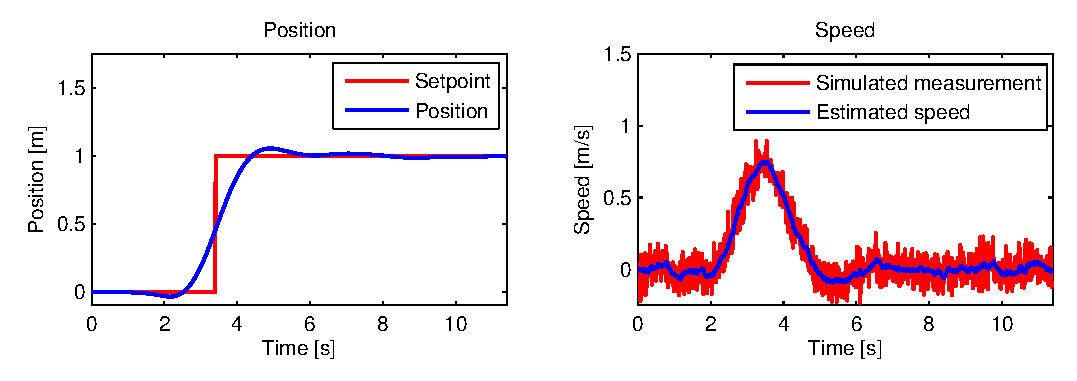
\includegraphics[width=0.99\textwidth]{fig/simulation1_step_no_governor.eps}
\caption{Simulating position step response without the input governor.}
\label{fig:simulation_step_no_governor}
\end{figure}

\begin{figure}[H]
\centering
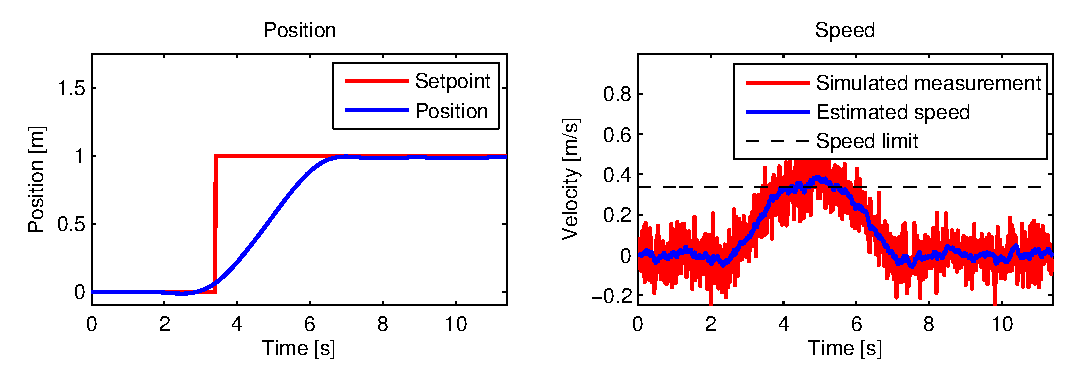
\includegraphics[width=0.99\textwidth]{fig/simulation2_step_governor.eps}
\caption{Simulating position step response with the input governor.}
\label{fig:simulation_step_governor}
\end{figure}

Since the desire \emph{unit step} trajectory is not feasible, it should be firstly transformed using the input governor. In our case, we limit the UAV's speed to $0.35\jed{ms^{-1}}$. Figure \ref{fig:simulation_step_governor} shows the Simulation of step response with the input governor. See that the speed lies roughly under the limit. 

\begin{figure}[H]
\centering
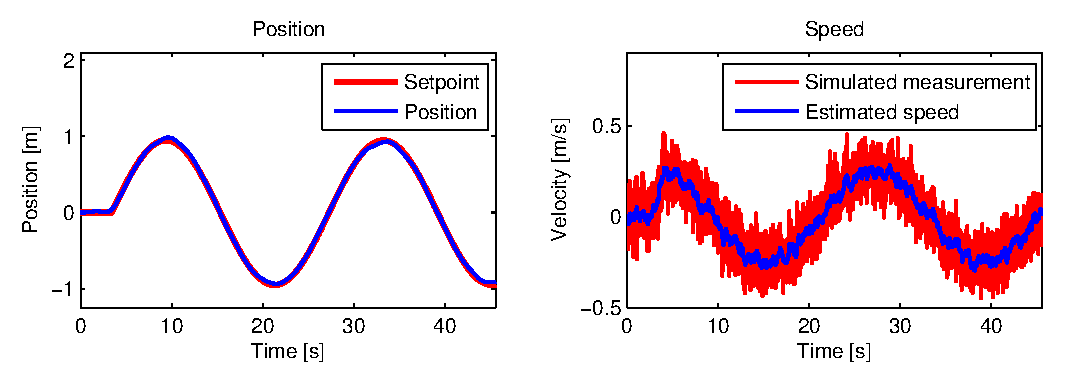
\includegraphics[width=0.99\textwidth]{fig/simulation3_sine.eps}
\caption{Simulating trajectory of feasible sine trajectory.}
\label{fig:simulation_step_governor}
\end{figure}

\begin{figure}[H]
\centering
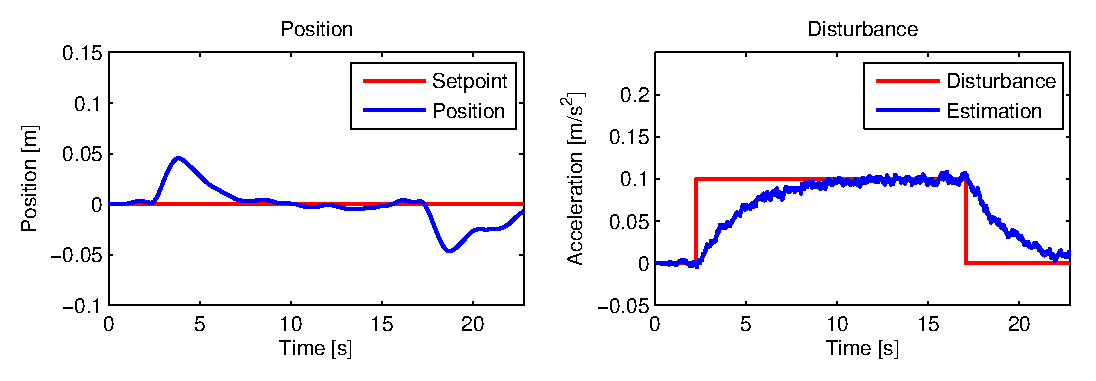
\includegraphics[width=0.99\textwidth]{fig/simulation4_disturbance_rejection.eps}
\caption{Simulating of disturbance rejection.}
\label{fig:simulation_step_governor}
\end{figure}

\subsection{Tracking constant setpoint}

\begin{figure}[H]
\centering
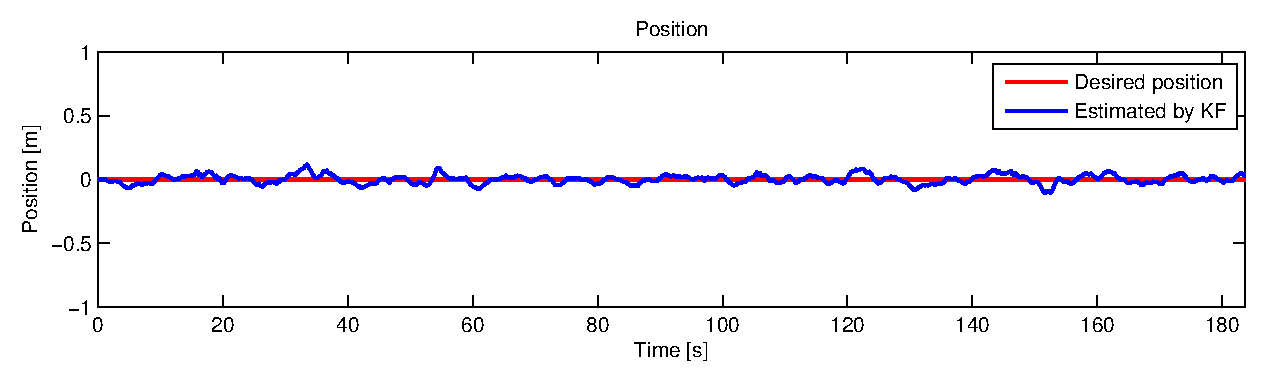
\includegraphics[width=0.99\textwidth]{fig/experiment6_constant_reference.eps}
\caption{Experiment with tracking static trajectory.}
\label{fig:experiment_sine_1}
\end{figure}

\subsection{Estimation drift}

\begin{figure}[H]
\centering
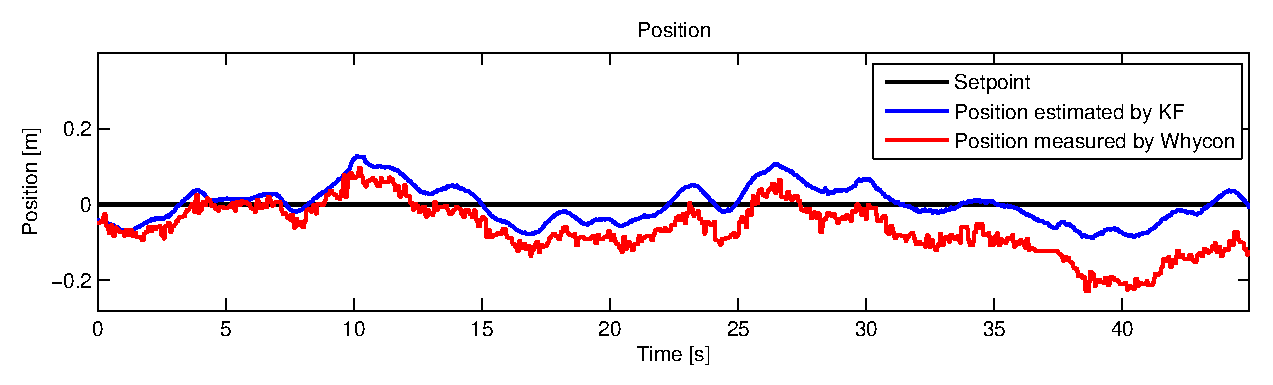
\includegraphics[width=0.99\textwidth]{fig/experiment5_drift_constant.eps}
\caption{Experiment with tracking static trajectory.}
\label{fig:experiment_sine_1}
\end{figure}

\begin{figure}[H]
\centering
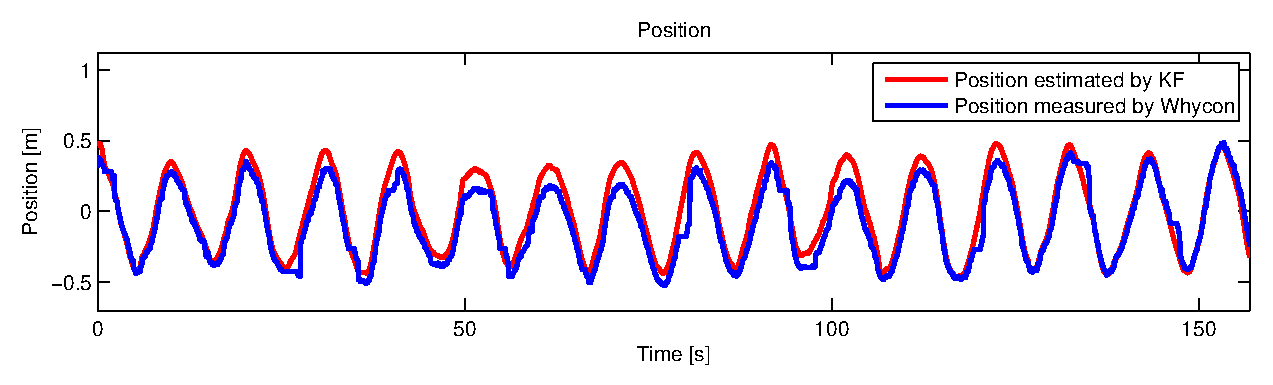
\includegraphics[width=0.99\textwidth]{fig/experiment5_drift_sine.eps}
\caption{Experiment with tracking sine trajectory.}
\label{fig:experiment_drift_sine}
\end{figure}

\subsection{Tracking dynamic trajectory}
\label{cap:dynamic_trajectory_tracking}

\begin{figure}[h]
\centering
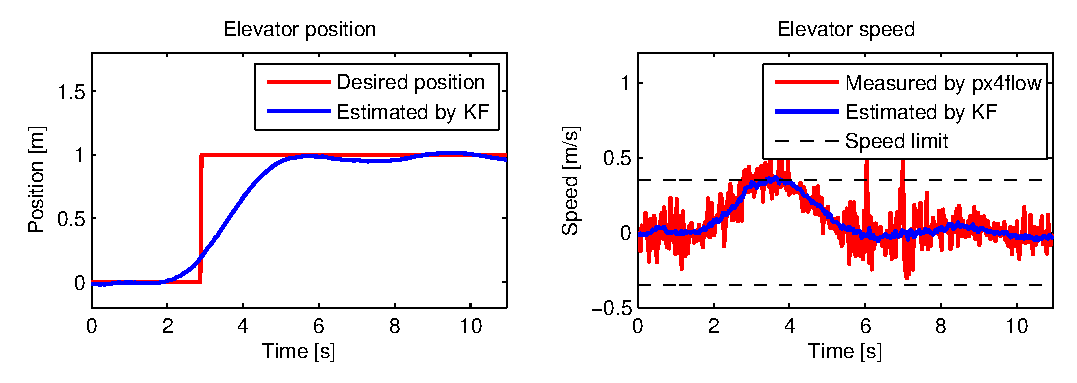
\includegraphics[width=0.99\textwidth]{fig/experiment2_step.eps}
\caption{Experiment with step response.}
\label{fig:experiment_sine_1}
\end{figure}

\begin{figure}[H]
\centering
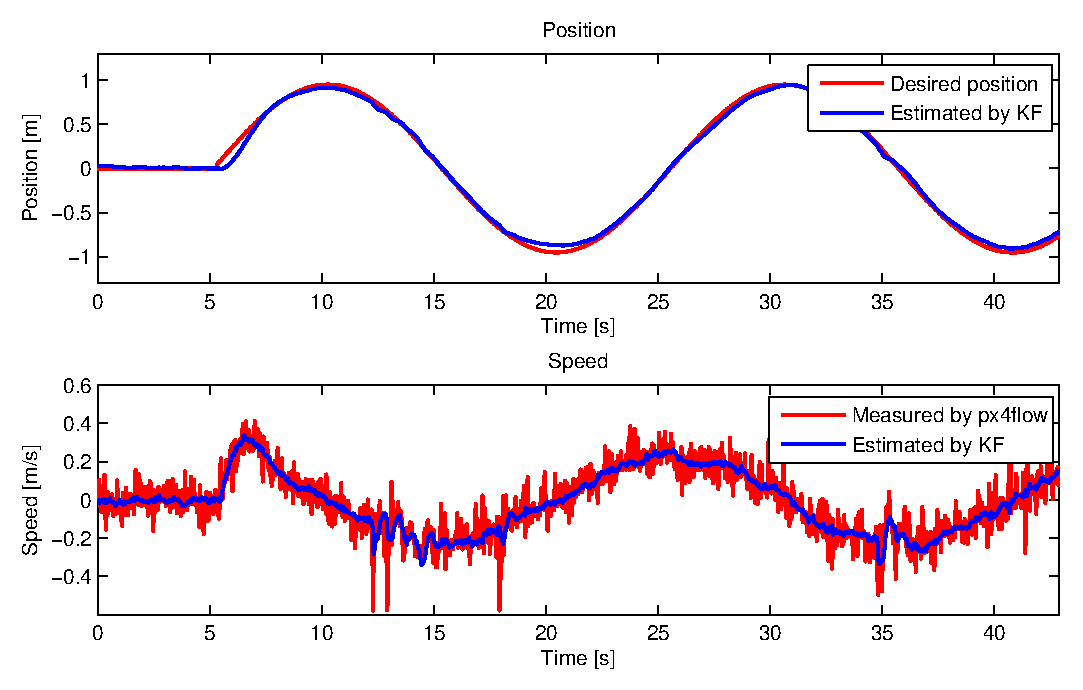
\includegraphics[width=0.99\textwidth]{fig/experiment1_sine.eps}
\caption{Experiment with tracking circular trajectory. Figures show position and velocity in single axis. Amplitude $0.95\jed{m}$, period $20\jed{s}$.}
\label{fig:experiment_sine_1}
\end{figure}

\subsection{Disturbance rejection}

\begin{figure}[H]
\centering
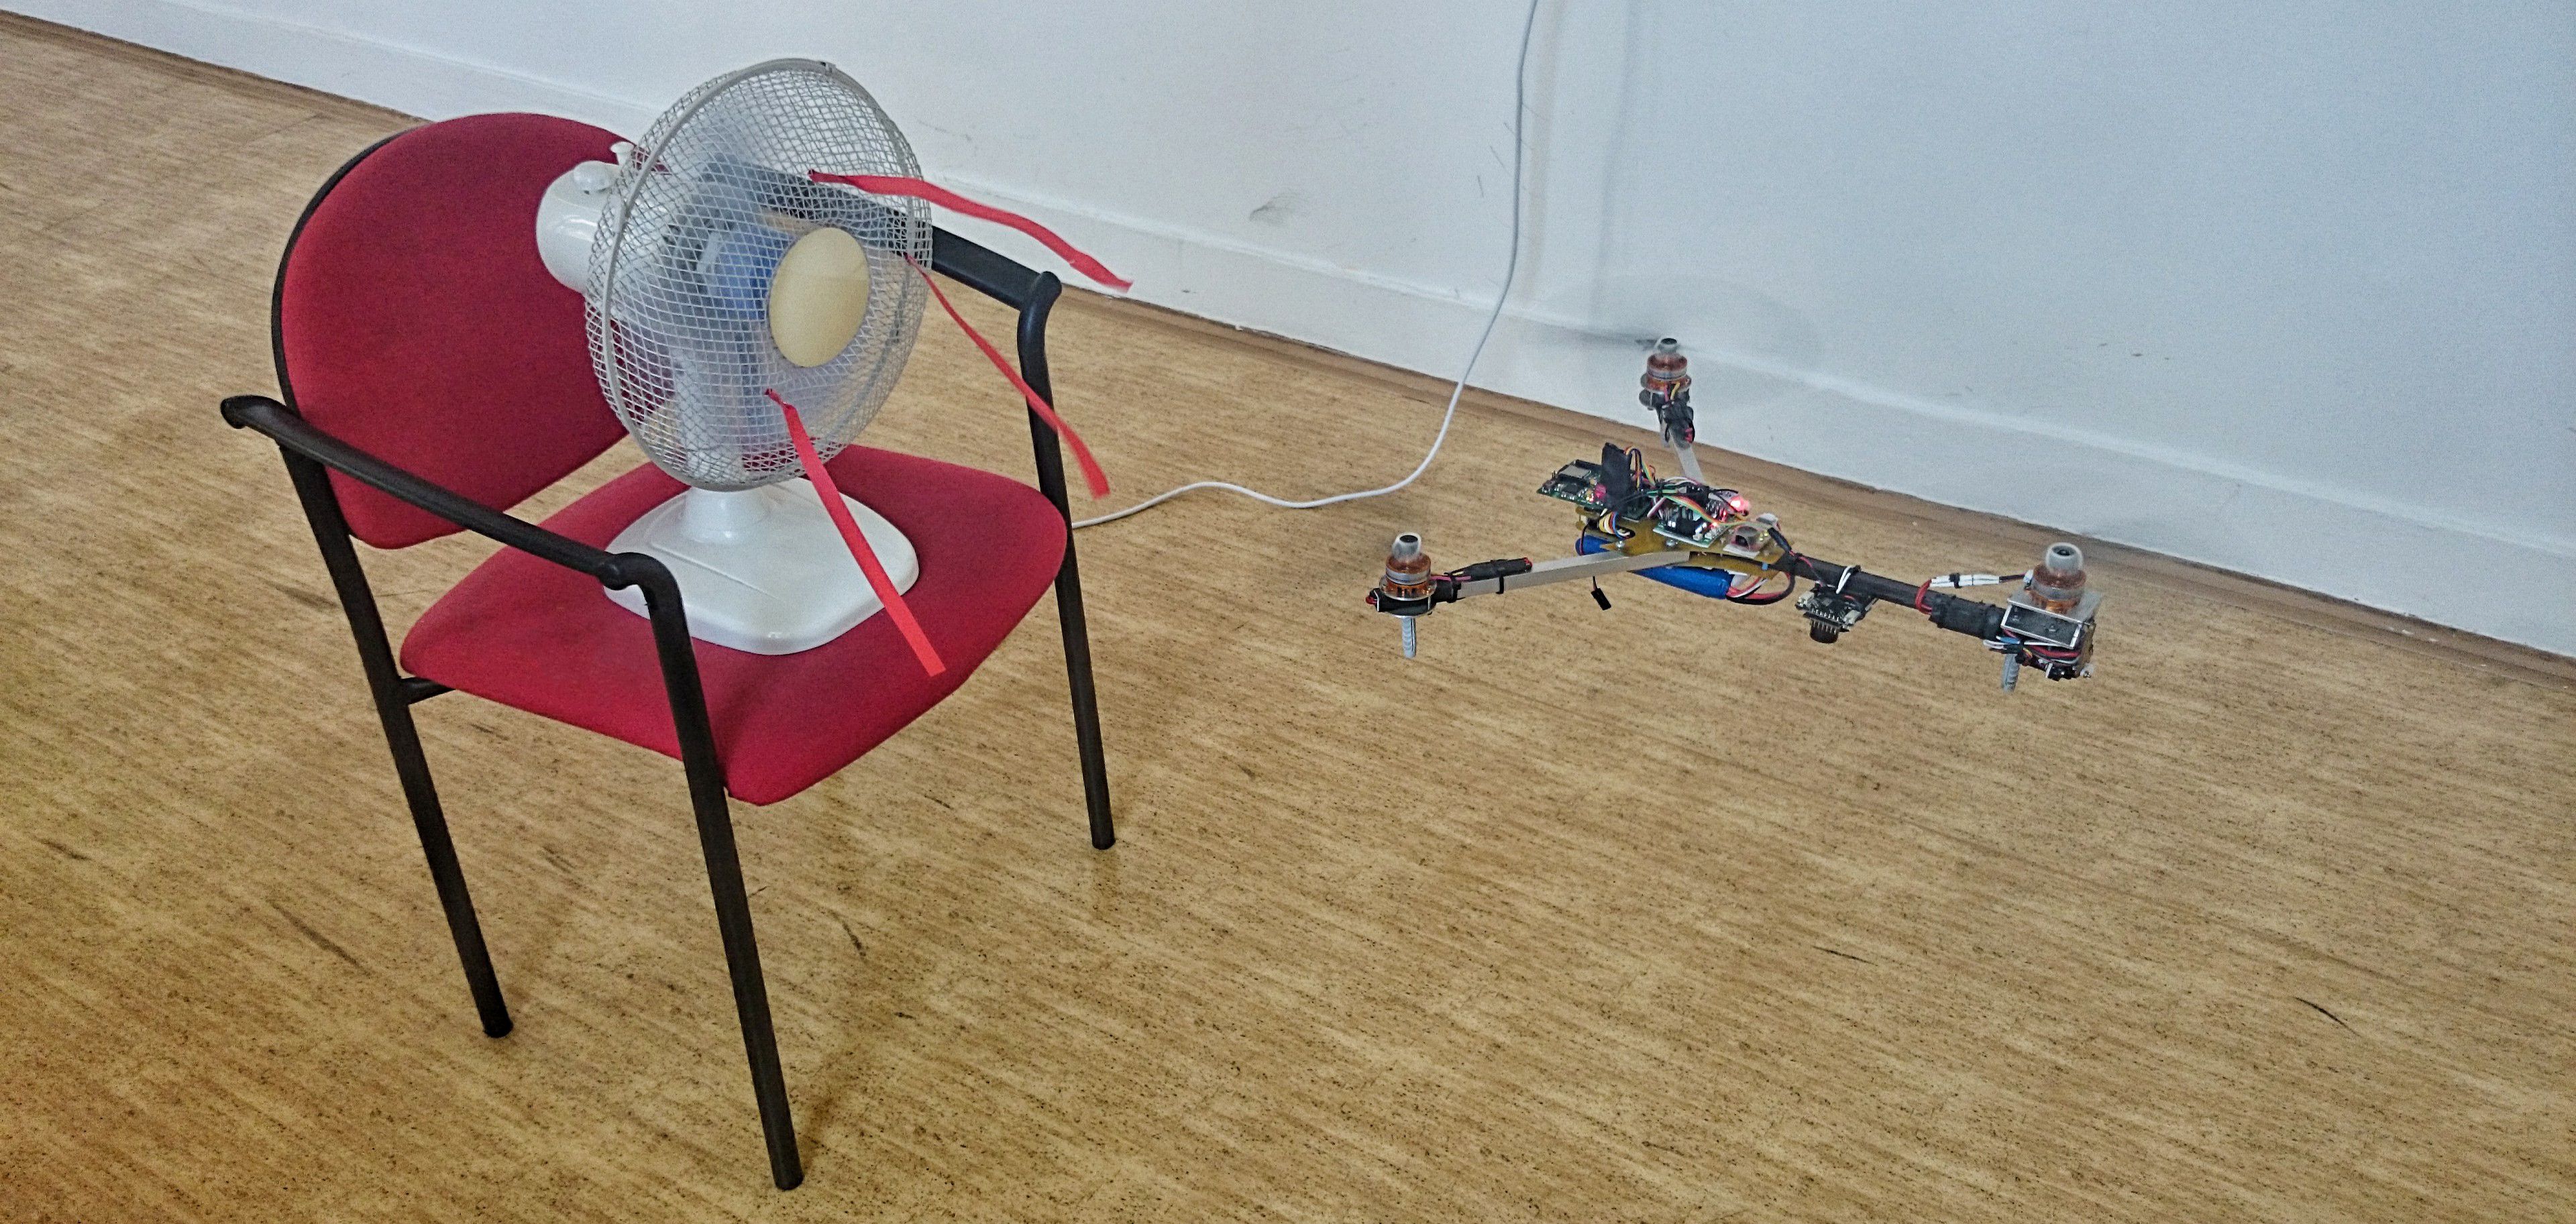
\includegraphics[width=0.99\textwidth]{fig/disturbance.jpg}
\caption{}
\label{fig:vetrak1}
\end{figure}

\subsubsection{Persistent wind disturbances}

\begin{figure}[H]
\centering
	\begin{tikzpicture}
		\node[anchor=south west,inner sep=0] (a) at (0,0) {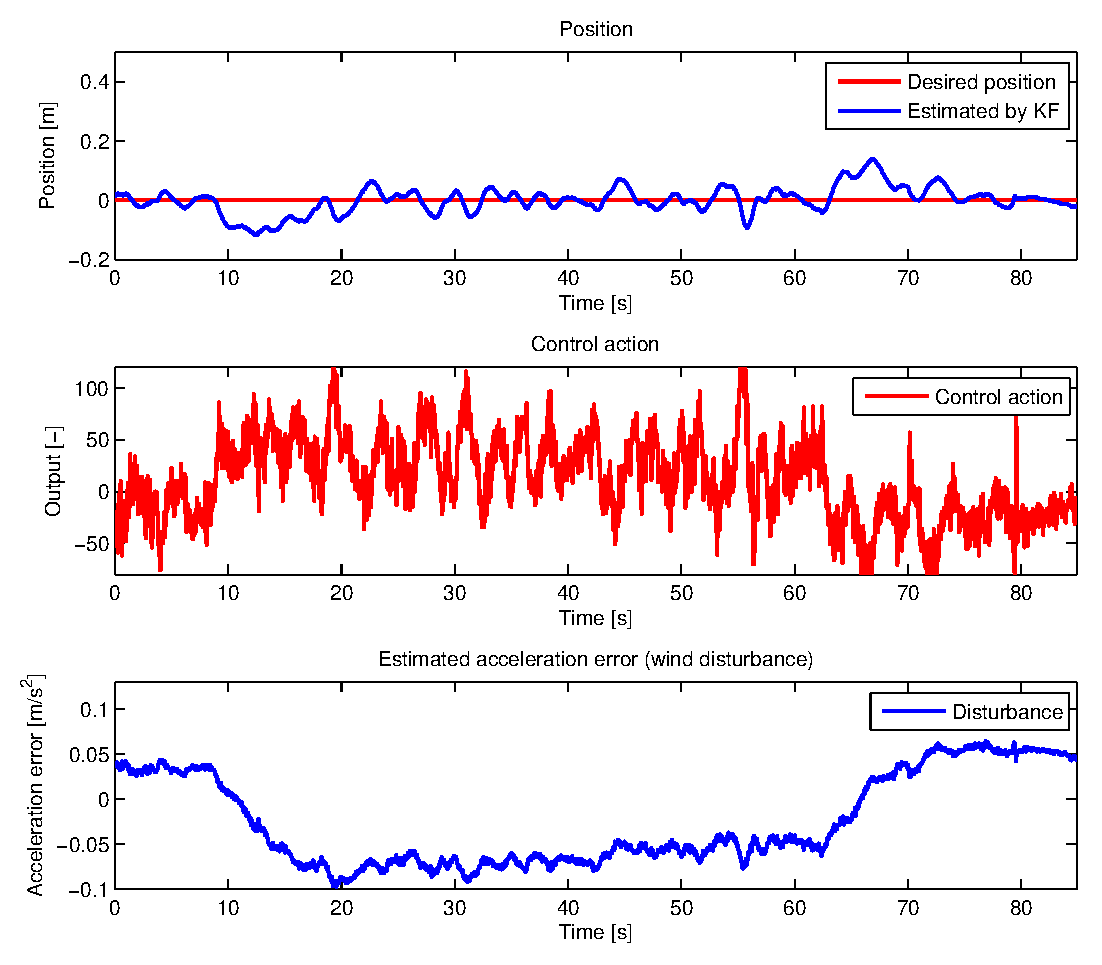
\includegraphics[width=\textwidth]{fig/experiment3_steady_disturbance.eps}};
		\begin{scope}[x={(a.south east)},y={(a.north west)}]

		%\draw[help lines,xstep=.1,ystep=.1] (0,0) grid (1,1);	
		
%        \draw[white,ultra thick,rounded corners] (0.55,0.50) rectangle (0.7,0.7);
%        \draw (0.58,0.655) node [text=white] {\textbf{1}};
        

		%\draw[-latex] (0.2,0.9) -- (0.2,0.81);    
		%\node[] at (0.25,0.92) {Disturbance started};    
		
		%\draw[-latex] (0.75,0.9) -- (0.795,0.81);    
		%\node[] at (0.65,0.92) {Disturbance went off};  
		
		\draw[fill=gray, opacity=0.2] (0.2,0.740) rectangle (0.757,0.960);  
		
		\draw[fill=gray, opacity=0.2] (0.2,0.401) rectangle (0.757,0.624);  
		
		\draw[fill=gray, opacity=0.2] (0.2,0.064) rectangle (0.757,0.286);  
        
    \end{scope}
	\end{tikzpicture}
\caption{Experiment with tracking constant setpoint while being under the influence of wind.}
\label{fig:experiment_steady_wind}
\end{figure}

\subsubsection{Momentary disturbances}
\label{cap:momentary_disturbances}

\begin{figure}[H]
\centering
	\begin{tikzpicture}
		\node[anchor=south west,inner sep=0] (a) at (0,0) {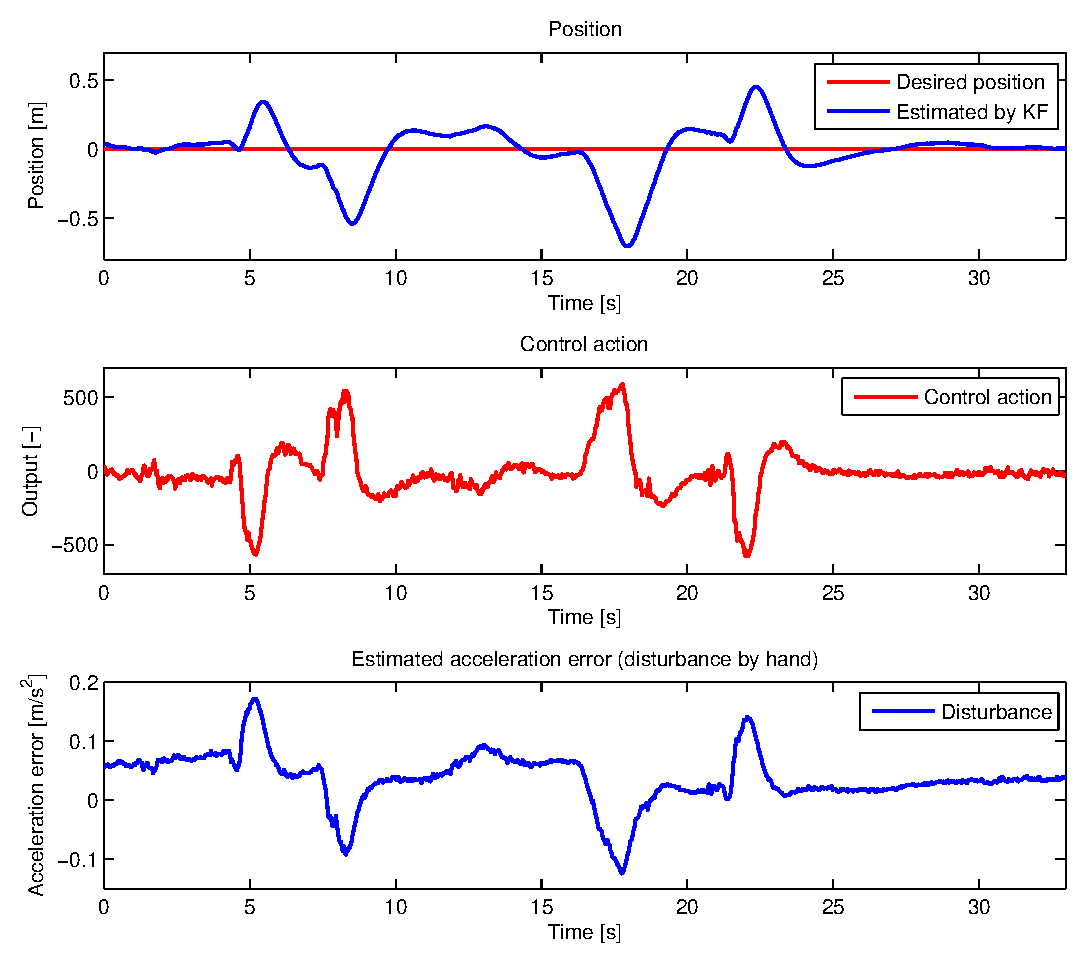
\includegraphics[width=\textwidth]{fig/experiment4_sudden_disturbances.eps}};
		\begin{scope}[x={(a.south east)},y={(a.north west)}]

%		\draw[help lines,xstep=.1,ystep=.1] (0,0) grid (1,1);	
		
%        \draw[white,ultra thick,rounded corners] (0.55,0.50) rectangle (0.7,0.7);
%        \draw (0.58,0.655) node [text=white] {\textbf{1}};
        

		\draw[fill=gray, opacity=0.2] (0.205,0.739) rectangle (0.235,0.9615);  
		\draw[fill=gray, opacity=0.2] (0.29,0.739) rectangle (0.319,0.9615);  
		\draw[fill=gray, opacity=0.2] (0.41,0.739) rectangle (0.445,0.9615);  
		\draw[fill=gray, opacity=0.2] (0.532,0.739) rectangle (0.575,0.9615);  
		\draw[fill=gray, opacity=0.2] (0.675,0.739) rectangle (0.7,0.9615); 
		
		\draw[fill=gray, opacity=0.2] (0.205,0.4015) rectangle (0.235,0.624);  
		\draw[fill=gray, opacity=0.2] (0.29,0.4015) rectangle (0.319,0.624);  
		\draw[fill=gray, opacity=0.2] (0.41,0.4015) rectangle (0.445,0.624);  
		\draw[fill=gray, opacity=0.2] (0.532,0.4015) rectangle (0.575,0.624);  
		\draw[fill=gray, opacity=0.2] (0.675,0.4015) rectangle (0.7,0.624); 
		
		\draw[fill=gray, opacity=0.2] (0.205,0.063) rectangle (0.235,0.286);  
		\draw[fill=gray, opacity=0.2] (0.29,0.063) rectangle (0.319,0.286);  
		\draw[fill=gray, opacity=0.2] (0.41,0.063) rectangle (0.445,0.286);  
		\draw[fill=gray, opacity=0.2] (0.532,0.063) rectangle (0.575,0.286);  
		\draw[fill=gray, opacity=0.2] (0.675,0.063) rectangle (0.7,0.286); 
        
    \end{scope}
	\end{tikzpicture}
\caption{Experiment with tracking constant setpoint while being under the influence of momentary disturbances. The UAV was dragged by hand.}
\label{fig:experiment_steady_wind}
\end{figure}

\subsection{Summary and comparison with previous work}